\section*{Results}

\subsection*{Two traits}

With two traits, trait evolution followed patterns associated with the type 
of tradeoff the two traits had when evolved together
(i.e., with the value of $\eta$)
(Figure \ref{fig:two-trait-outcomes}).
When the tradeoff is sub-additive ($\eta = -0.6$), there is a single
stable point in the trait space, where both traits are
maximized---within the limits imposed by traits' negative effects on 
the growth rate.
When the tradeoff is super-additive ($\eta = 0.6$), there are two
alternative stable states, one for each trait being maximized while the 
other is zero.
Lastly, when the tradeoff is additive ($\eta = 0$), traits
evolve to any point on a neutrally stable ring.


\begin{figure}[ht!]
\centering
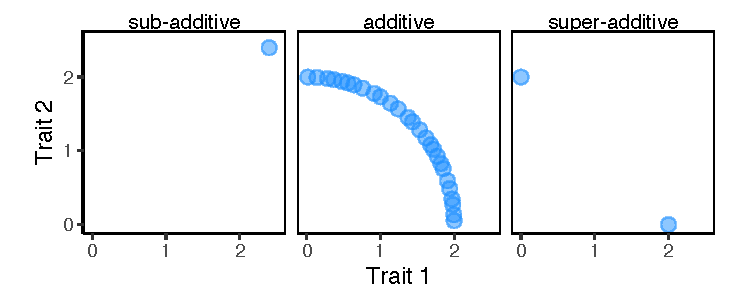
\includegraphics{1-outcomes_q2.pdf}
\caption{Unique trait values for surviving species in simulations of 2-trait communities,
    for tradeoffs being sub-additive, additive, or super-additive.}
\label{fig:two-trait-outcomes}
\end{figure}


For communities containing species with widely varying starting trait values,
coexistence occurs only when evolution for all traits is non-conflicting
(Figure \ref{fig:coexist}A),
and a value of 0 for any $d$ appears to represent a threshold with respect 
to whether coexistence can occur (Figure \ref{fig:coexist}B).
Even slightly negative values of $d$ cause exclusion to occur, although
a less-negative $d$ causes the exclusions to happen more slowly
(Figure \ref{fig:coexist}C).



Super-additivity can lead to multiple possible trait states in a 
community.
When species start with trait values that vary widely 
across the trait space, both trait states can be occupied 
simultaneously only when evolution for both traits is non-conflicting.
However, when one trait is non-conflicting and all starting
trait values in the community lie in the basin of attraction
for that trait being maximized, then coexistence can occur
(Figure \ref{fig:cond-coexist}).
Thus, even in this simple case, community evolution can follow
one of two paths depending on starting conditions:
One species evolves fastest to the conflicting state and 
excludes others, or
multiple species evolve to the non-conflicting state
and coexist.


\begin{figure}[ht!]
\centering
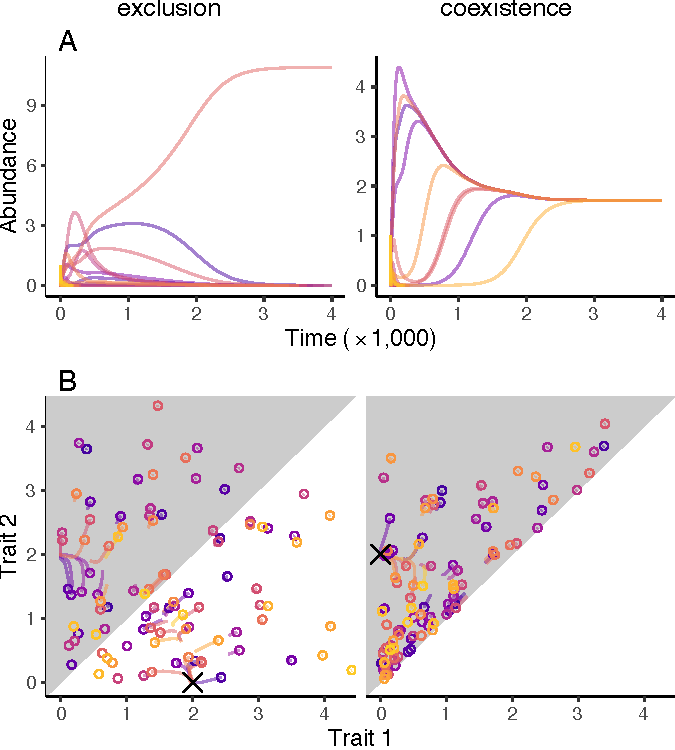
\includegraphics{2-cond_coexist.pdf}
\caption{Two simulations illustrating conditional coexistence for one
    conflicting and one non-conflicting trait.
    The left panels show exclusion, whereas the right show
    conditional coexistence.
    In the top two panels, each line is for a particular species.
    In the bottom two panels, circles show starting trait values,
    and lines show trajectories through trait space through time.
    Xs show the trait values for surviving species.
    The gray area is the basin of attraction for the
    non-conflicting trait.
    Here, $d_1 = d_2 = 0.1$}
\label{fig:cond-coexist}
\end{figure}




\subsection*{Three and four traits}


Many more patterns of possible trait states existed for the 3-trait case
(Figure \ref{fig:three-trait-outcomes}).
Similar to 2 traits, all sub-additive tradeoffs resulted in 1 stable state, and
all super-additive tradeoffs resulted in $q$ stable states.
Only one state existed when two or more tradeoffs were sub-additive,
except when the tradeoff with the highest magnitude was super-additive while
the others were sub-additive.
Additivity in one trait often, but not always, resulted in a portion of a
neutrally stable ring being ``available'' for surviving species.
When no traits were sub-additive, part of a neutrally stable ring
always represented the potential trait states.
When all traits were additive, traits existed along a neutrally stable 
three-dimensional shell.




\begin{figure}[ht!]
\centering
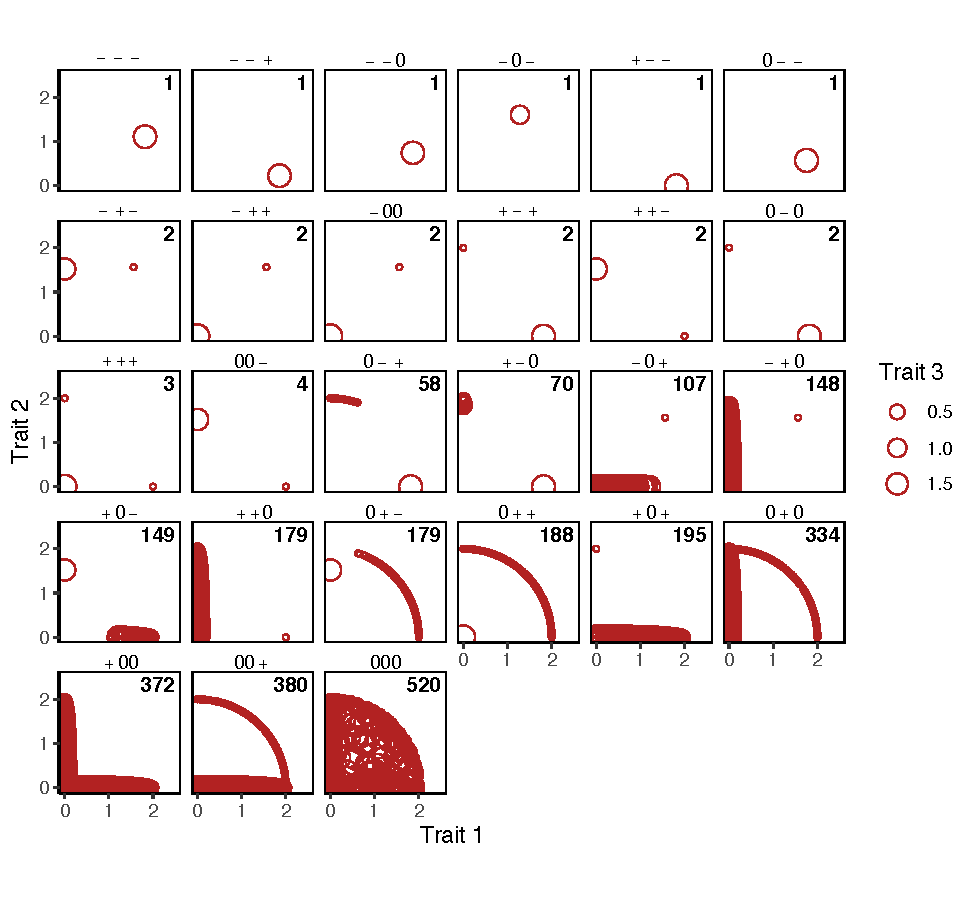
\includegraphics{3-outcomes_q3.pdf}
\caption{Unique trait values for surviving species in simulations of 3-trait communities,
    for all 27 permutations of tradeoffs being sub-additive (``$-$''), additive (``$0$''),
    or super-additive (``$+$'').
    The point size indicates the value of trait 3.
    Numbers in the corner of each panel indicate the number of unique trait states
    for that particular permutation, and panels are arranged by this number.
    For these simulations, the magnitudes of the $\eta$ values were 
    $0.1487$ for $\eta_1$, $0.3423$ for $\eta_2$, and $0.1118$ for $\eta_3$.}
\label{fig:three-trait-outcomes}
\end{figure}







\textbf{\textit{To-Do List:} }
\begin{itemize}
\item Should I do another set of simulations similar to those in figure
    \ref{fig:three-trait-outcomes}, but with $d = 0.1$? If you recall, some
    of the alternative trait states didn't exist when $d = 0.1$.
\item Joe mentioned simulating 4 traits, one or more of which is conflicting,
    because the number of tradeoffs is greater than the number of traits,
    and this might allow for coexistence.
\item I should include $N$ in the Jacobian because, as it stands, the Jacobians
    tell me nothing about whether more species will go extinct.
\end{itemize}

